\chapter{Adapt to Frequent Network Failure and Limited Bandwidth}\label{sync}
In this chapter, problems are further decomposed and analyzed. To prevent reinventing-the-wheel, a variety of possible solutions are proposed and investigated, whereas focus has been put into our unique requirements.

%Most of techniques today focus on reducing response time and improving concurrency, rather than offline operation and network partitioning. Even though major companies optimize their server architecture for miliseconds of faster, web service in rural areas is still a question of existance.

%TODO Read-only and Read-write

%Overall goals are:
%\begin{itemize}
%\item To reduce user-perceived latency and bandwidth usage within the context of rural LAN with a narrow upper link.
%\item To serve up-to-date content.
%\item To achieve partition tolerance by continuing service when network failure occurs.
%\end{itemize}

\section{A closer look at the problem} \label{components}
As introduced in section \ref{out_intro}, Moodle is deployed as underlying course management system for OUT E-learning platform. Moodle is an open sourse project written in PHP and well-documented\cite{aosamoodle}\cite{moodledoc}. Similiar to other web applications, it can be deployed in a typical LAMP or LNMP stack. In this chapter, we mainly focus on possible solutions for two problems stated previously, and leave the choice of actual server to chapter \ref{benchmark}

%Moodle components
Moodle is a typical database-driven web application where all the pages are generated on-the-fly based on user request. The whole application is composed of three main components: 
\begin{itemize}
\item PHP source code, typically in \texttt{/var/www/moodle/}
\item A database to store data or metadata including site configuration, student information, course details, events, etc. There exist volatile tables in Moodle database which store sessions and temparory information.
\item A directory to store materials and resources, as well as cache and temparory files. Typically it is named as \texttt{moodledata/}
\end{itemize}

%model of problem
The problem addressed previously can be simplified and modelised as following,
see Figure \ref{problem_model}. Each node in the model denotes a local
server/proxy and has a certain amount of users associated with it.

\begin{figure}[htbp]
\centering
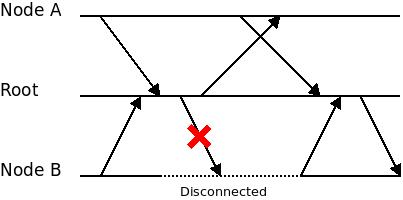
\includegraphics[width=0.6\textwidth]{../images/model_centralized.jpeg}
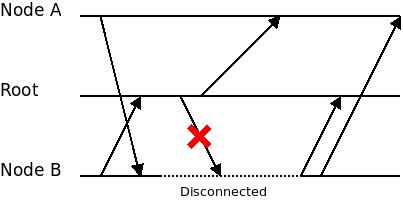
\includegraphics[width=0.6\textwidth]{../images/model_distributed.jpeg}
\caption{Web Delivery Model}
\label{problem_model}
\end{figure}

%What to store
As simple as the model might be, components in it could be vastly heterogenous if mapped to different techniques. Content stored in a node can either be web objects, SQL replies, codes or even entire databases. Communication in between can also be based on a variety of protocols.

%Interactive session
As an online learning platform, users do not only passivly accept information, but also interact with Moodle through forum, personal blogs and quiz. All the changes made by users must be stored and seen everywhere. Thus, the system should not be read-only under any circumstance.

%Dynamic content


%production and minimum affection
Moodle has been in service and adding new services should affect existing structure as less as possible. Also, steps of adapting changes should be properly designed to avoid crushing the service.

%communication overhead
To maintain consistency and serve up-to-date content, a reasonable amount of
communication overhead is necessary and is normally positive proportional to the
extent of consistency. Although, due to the presumption of poor network
connection and narrow bandwidth, different nodes in the system are preferably
decoupled and autonomous.

%Offline operation
The autonomy is also closely correlated to the ability of performing offline operation. Many distributed systems have the ability to detect and recover from network partitioning, although it normally leads to a compromise of consistensy and content freshness. When a user request a page, Moodle loads all previliges of the user, generate pages accordingly and log the session. This results in uncacheble content and interaction-must logins. It has been proven that consistency, high availability and partition tolerence are impossible to be achieved at same time\cite{brewer2000towards}\cite{gilbert2002brewer}, necessary trade-off has to be made according to the condition and needs.

While the majority of web caching and content distribution techniques aim at better performance and delivery efficiency, we prioritize the ability of performing basic functionalities during network failure. We tolerate a relatively loose consistency while ensuring eventual convergence.

%Affordability
Lastly, to realize affordability, we mainly focus on open source techniques and free ware. Thankfully, many successful projects and tools have been made open source and publicly available. In the following sections of this chapter, we evaluate a variety of techniques against the criteria stated above and propose our solution based upon the conclusion. Several of potential solution are also tried out.


\section{Push Web Service to Edge}
\subsection{Content Delivery Network}
Content Delivery Network overlaps with Web Cache Proxy at the concept of pushing web content to users. A Content Delivery Network is a collaborative set of surrogate servers spanning the network, where web contents are mirrored\cite{pathan2008content}. Users will perceive a smaller latency while fetching content from a nearby CDN surrogate server rather than original web server. The essence of CDN is illustrated in Figure \ref{cdn}.

\begin{figure}[htbp]
\centering
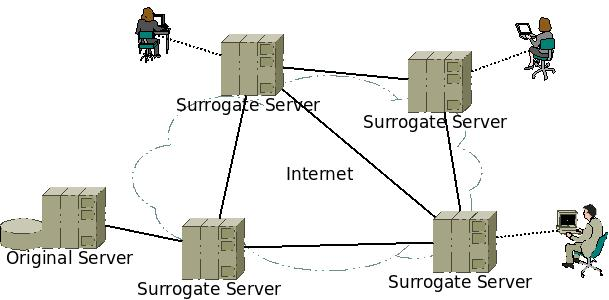
\includegraphics[width=0.8\textwidth]{cdn.jpeg}
\caption{Content Distribution Network}
\label{cdn}
\end{figure}

Since more and more web services are evolving to provide dynamic content, CDN also takes advantages of cachebility hints when dealing with dynamic contents\cite{dilley2002globally}. 

%TODO open source CDN project

\subsection{Simple Web Caching}
An intuitive and common solution for the problem of limited bandwidth is to cache popular web content locally, as illustrated in Figure \ref{with_cache}.
A client-side web cache proxy is typically deployed in user local network, requesting web servers on behalf of users, and cache web objects for further references. Web caching has been proven to be an effective approach to reduce bandwidth usage, user-perceived latency and loads on original server\cite{davison2001web}.

\begin{figure}[h]
\centering
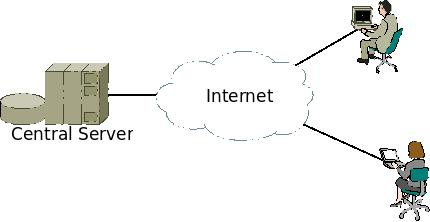
\includegraphics[width=0.6\textwidth]{../images/without_caching.jpeg}
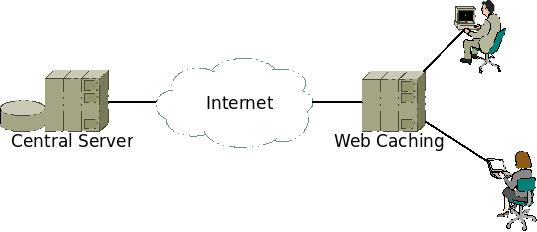
\includegraphics[width=0.6\textwidth]{../images/with_caching.jpeg}
\caption{Serve users without and with a Gateway Cache}
\label{with_cache}
\end{figure}

Web cache is greatly advantageous in our scenario that it does not require modification on web application, except that some TCP optimizations could be done between web cache proxy and web server frontend. Web cache proxy can continue serving requests with offline mode enabled, which also meets our requirements. The traffic between cache proxy and authentic server is standard HTTP request and response. The overhead and frequency of communication mainly depends on cache hit / cache miss ratio, expiration time and cache directory size.

Although, this solution encounters two major constraints in our case:
\begin{itemize}
\item Moodle pages are generated on-the-fly based on user information. Web cache cannot operate on its own during network failures, except for serving previously requested pages.
\item Users are required to log in to browse. Thus, user-server interactions are always necessary, which also contradict with our purposes.
\end{itemize}

%One important feature of all web cache proxies is replacement strategy which invalidate caches and maintain freshness. A comprehensive survey of existing replacement strategy is presented in \cite{podlipnig2003survey}. However

\subsection{Page generation on Edge Server}
To address the issue of dynamic content generation and client-server interaction, an intuitive and brute-force solution is to generate user-specific page at the edge. A comprehensive study of edge servers can be found in \cite{pathan2008content}. Four strategies are presented: (a) edge computing (b) content-aware caching (CAC) (c) content-blind caching (CBC) (d) data replication.
%TODO replication figure
In each of the strategy, the edge server attempts to reply user request on the behalf of original server with the information that is locally available. Edge computing still heavily relies on central database, hence out of our consideration. While CAC and CBC store partial database at the edge, data replication stores a complete copy of the database.

If the size and complexity of database permit, data replication is desired since it outperforms other strategies in both response speed and offline operation. Although, it adds another layer of complexity to perform transaction processing and maintain the consistency through mutliple distributed databases. Techniques to achieve a consistent distributed database system are presented in section \ref{database_sync}.

Application code rarely changes in our case and is always one-way synchronized from original server, thus consistency can be relatively easy to achieve by periodically utilizing tools like rsync\cite{tridgell1999efficient}.

%TODO file system

\section{Multi-Master Database Synchronization} \label{database_sync}
As addressed previously, consistency, availability and partitioned-network cannot be accomplished at the same time, according to CAP theorem\ref{brewer2000towards}. Necessary trade-off has to be made to adapt to particular circumstance. Based on objectives defined previously, we prioritize availability and partitioned-network, while allowing loose consistency, as long as eventual consistency is guaranteed\ref{vogels2009eventually}. Pessimistic replication always guarantees consistent content perceived by users, thus widely adopted in distributed database system to enhance availability and performance. Although optimistic replication permits diverged databases, which is more suitable in our case. An exhaustive survey on optimistic replication is presented in \ref{saito2005optimistic}.

Comprehensive theoretical researches have been made available although we find limited open source implementations that serve our purposes. We investigate several data replication technologies in this section based on following criteria:
\begin{itemize}
\item \textbf{Deployable over WAN}
Most of distributed database system assumes a LAN environment, where delay and bandwidth do not evidently affect exchange of data among servers. Although in our case, databases are deployed over WAN, which is highly unreliable and network latency is not neglectable.

\item \textbf{Serializibility}
To achieve eventual consistency, concurrent changes made at different edge servers need to be serialized. Hence, an order of operations is extracted based on relations among them.

\item \textbf{Conflict detection and reconsiliation}
\end{itemize}

 Several data replication technologies are investigated in this section in order to find a tool that requires minimum modifications to fit into our problem.

Distributed database system is widely adopted in server clusters and workstations, as a mean to enhance performance and redundancy. Although LAN is normally assumed by most of database replication technologies. 





%Database replication techniques has been intensively deployed over clusters and workstations for redundency and load balancing. A LAN is always assumed by most of database replication techniques, whereas database replicas across the WAN are desired to realize our goals. We prioritize availability by compromising on consistency, as long as the system can reach eventual consistency\cite{vogels2009eventually}. Offline operations on distributed databases often encounter simutaneous modification on the same entry, which result in conflict after reconnection. Techniques to detect and reconsile conflicts are studied and evaluated.
%TODO transaction process

\subsection{Database Cluster} \label{db_cluster}
%CouchDB
\textbf{CouchDB}\cite{couchdb} is an open source distributed database system developed in Apache. The most attractive feature of CouchDB is that it natively supports bi-directional synchronization among multiple database replicas and offline operations. When one replica is disconnected from the network, it retains autonomy and continues as a fully functional database from user point of view. Although, it fails to be our candidate since it is NoSQL database, whereas Moodle heavily relies on SQL calls and it will a significant task to modify Moodle to use NoSQL database.

%MySQL native replication
\textbf{MySQL Native Replication} is shipped with most of MySQL standard distributions that provide built-in functionalities to replicate databases. The synchronization is uni-directional that databases on master node are replicated to slave nodes. ALthough bidirectional synchronization can be achieved by creating loop in the topology. A simplest 2-nodes example can be found in Figure X. Node A and node B synchronize with each other by maintaining mutual dominance. The figure also shows a more complicated topology where three nodes comprise a loop. Although, the synchronization can be easily broken by conflict and the reconciliations always require human intervention.
To avoid insertion conflicts of auto-incremental keys, MySQL provides an option to increase incremental step. This feature is further discussed in section \ref{multi_master}

\begin{figure}[htbp]
\centering
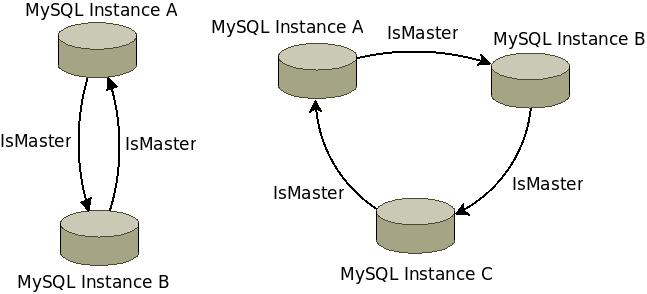
\includegraphics[width=0.7\textwidth]{mysql_repl.jpeg}
\caption{MySQL Replication}
\label{mysql_repl}
\end{figure}

%MySQL cluster
\textbf{MySQL Cluster}\cite{mysqlcluster} is an open source distributed database system based on MySQL. It supports database sharding and duplicating. A typical use case of MySQL Cluster is shown in Figure \ref{mysql_cluster}. Although, redundent copy of database can only be accessed with the presence of management master, and cannot be updated during network failures. Furthermore, database nodes are closely coupled with the assumption of LAN (low latency and high bandwidth).

\begin{figure}[htbp]
\centering
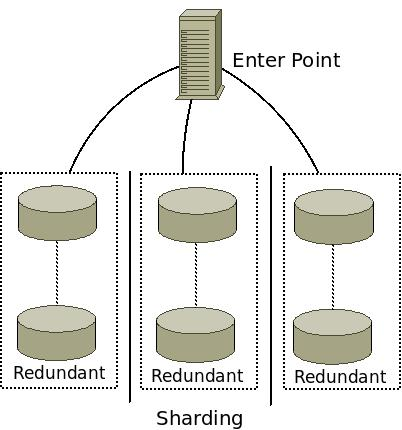
\includegraphics[width=0.4\textwidth]{mysql_cluster.jpeg}
\caption{MySQL Cluster}
\label{mysql_cluster}
\end{figure}

\subsection{Middleware-based Repliation System}
Several studies also proposed the approaches to solve database synchronization at middleware-level\cite{cecchetc}\cite{amza2003conflict}\cite{plattner2004ganymed}. C-JDBC \cite{cecchetc} is an Java implementation of RAIDb\cite{cecchet2005raidb}, aiming at a framework to manage heterogenous databases. With built-in functionality of scheduling transaction processes, C-JDBC is perceived by users as a single virtual database. Although, the system is still centrally managed and could not handle partitioned network. Ganymed middleware system\cite{plattner2004ganymed}, inspired by C-JDBC, achieves consistency by serializing update/write requests at master and propogating changes to replicas in a lazy fashion. Users see a consistent data state (snapshot isolation), even though stale might it be. The limitation of these two middleware is also clear, that no write can be served during network failures.


\subsection{Multi-Master Sycnhronization System} 
Similiar to MySQL Cluster Multi-Master setup, we found three state-of-the-art open source tools to the similiar end.
\begin{itemize}
\item \textbf{Galera}\cite{galera} is an open source synchronous database replication software developed to scale web application and provision high availability. It achieves consistency by optimistic locks and group communication. Galera is quorum-based and handles network partitioning by sacrificing the minority. Hence, Galera lacks the essencial features that we are seeking for and is out of consideration.
\item \textbf{Tungsten}\cite{tungsten} replicates database asynchronously and allows loose consistency. Transactions are commited locally, and then propogated across all other nodes. Tungsten features offline operation and automatical recovery although it leave the responsibility of conflict avoidance completely to the application. Conflicts may disturbe replication and hard to trace.
\item \textbf{SymmetricDS}\cite{symmetricds} is another open source asynchronous database replication management tool. It has several built-in rules to detect and reconsile conflicts. It can be configured flexibly to meet different needs, for example, have different courses store in different sites. Also, one appealing feature is that SymmetricDS support file synchronization as well. Figure \ref{symmetricds} birefly illustrates how SymmetricDS works and more details in terms of conflicts detection and reconsiliation are discussed in section \ref{multi_master}
\end{itemize}

\begin{figure}[htbp]
\centering
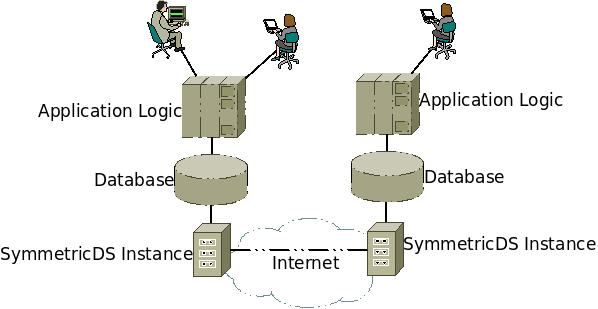
\includegraphics[width=0.8\textwidth]{symmetricds.jpeg}
\caption{SymmetricDS}
\label{symmetricds}
\end{figure}

We can conclude from above comparison that SymmetricDS is closest to our critaria and can be properly extended to meet our requirements. In the following section, we explore SymmetricDS in details and propose an approach to extend it.

\subsection{Conflicts Avoidance and Reconciliation} \label{multi_master}
Before we start illustrating our approaches for conflict detection and resolution, several reasonable application-specific assumptions need to be made:
\begin{itemize}
\item No user will attempt to login into two different server simutaneously, thus the content belong to this user will not be modified at two different sites.
\item Administration-related content is always synchronized through top-down approach, that is, user creation, deletion and modification are always synchronized in one-way.
\item No local user will be able to reply to a post that is not propogated to this edge server yet.
\item Volatile entries are not synchronized, such as cache and session.
\item Deletion wins. And events that causally follow the deletion also get deleted. If users reply to a post on a remote server whereas the post gets deleted on central server, all replies will get deleted once converged.
\end{itemize}

As introduced in section \ref{db_cluster}, insertion conflicts of primary keys can be avoided by setting different incremental steps, as long as the primary key is auto-incremented integer, see Table \ref{mysql_key_inc}.

\begin{table}[htbp]
\centering
\begin{tabular}{c|c|c|c}
Primary Key & Node A & Node B & Node C\\
\hline
1 & inseted by A & & \\
2 & & inserted by B & \\
3 & & & inserted by C \\
4 & inserted by A & & \\
5 & & inserted by B & \\
\end{tabular}
\caption{MySQL instances with different auto-incremental steps}
\label{mysql_key_inc}
\end{table}


Thankfully, all Moodle database tables are designed to use auto-incremental keys as primary key. By configuring incremental step and SymmetricDS, we are able to achieve a naive mutually consistent system. Configuring SymmetricDS is nontrivial and requires constant observation. Appendix A describes a work flow of configuring SymmetricDS.

Although, there are several major drawbacks of this design:
\begin{itemize}
\item It is not scalable. The incremental step limits the max number of servers in the system.
\item It is blind to application. It does not check logical correctness of modification according to application, e.g. replies to a previously deleted thread can still be inserted into database.
\end{itemize}

To attack these problems, we examine the way SymmetricDS handles conflicts and propose an extension that is more flexible and tunable. SymmetricDS applies the concept of CVS (Concurrent Versions System) to detect conflicts at a granularity of table entry level. When a node propogates a change on one table entry, it sends the before-state of that entry along with the change. Upon receipt, remote node compares the current state of this entry and the history. If they differ, a conflict is detected. Even though conflict resolution is highly application-specific, SymmetricDS provides limited rules to resolve known types of conflicts.

A SymmetricDS node can be configured to either actively pull from other nodes, or passively waiting for changes being pushed. While optimistic replications normally assume a negotiation phase while attempting a resolution, push and pull in SymmetricDS are independent from each other. Thus, conflicts resolution can be sometime confusing. For example, suppose a scenario in Figure \ref{sym_confuse}. Slave node is configured to push data to master while pulling changes from it. Since two operations are independent from each other, two replies to the same post are replaced by each other at two nodes, whereas the intention is to simply stack them.

\begin{figure}[htbp]
\centering
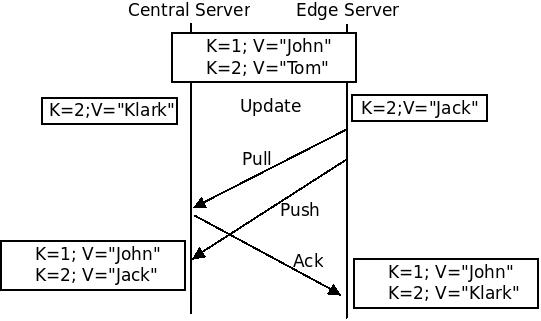
\includegraphics[width=0.8\textwidth]{sym_confuse.jpeg}
\caption{Misbahavior of SymmetricDS}
\label{sym_confuse}
\end{figure}

To attain serializibility, several repliation systems applies a centralized algorithm that serialize all changes at master node and then propogate to slaves. Although, it often requires a closely connected system and can suffer from latency and disconnection. Inspired by Git and Operational Transformation \cite{ellis1989concurrency}, we propose a distributed work flow in Figure X where conflicts are resolved at edge server, similiar to the mechanism used in Dropbox\cite{dropbox}. Edge node always pull the master first before commiting any changes. 
%TODO conflicts resolution work flow figure

